\documentclass[a4paper]{scrartcl}
\usepackage{amsmath,amssymb,amsthm}
\usepackage{bm}
\usepackage{biblatex}
\usepackage{float}
\usepackage[colorlinks=true, allcolors=black, urlcolor=cyan]{hyperref}
\usepackage{graphicx}
\usepackage{mathtools}
\usepackage[framed,numbered]{matlab-prettifier}
\usepackage{mcode}
\usepackage{physics}
\usepackage{siunitx}

\usepackage{todonotes}

\renewcommand{\thesection}{\arabic{section}}
\renewcommand{\thesubsection}{\arabic{section}\alph{subsection})}

\title{Assignment 1}
\subtitle{ELEC 442 - Introduction to Robotics}
\author{Sondre Myrberg}

\setlength{\parindent}{0pt} % Disable indentation
\mathtoolsset{showonlyrefs} % Only show equation numbers on referenced equations

\def\undertilde#1{\mathord{\vtop{\ialign{##\crcr
$\hfil\displaystyle{#1}\hfil$\crcr\noalign{\kern1.5pt\nointerlineskip}
$\hfil\widetilde{}\hfil$\crcr\noalign{\kern1.5pt}}}}} %Lousy way, but need this undertilde


\begin{document}

\hypersetup{pageanchor=false}
\begin{titlepage}
    \maketitle
    \vfill
    \vfill
    \vfill
    \vfill
    
\includegraphics[width=0.95\textwidth]{../../ubc_logo.pdf}
    \vfill
    \vfill
\end{titlepage}
\hypersetup{pageanchor=true}

\section{}  

Given the homogenous transformation
\begin{equation}
    \begin{bmatrix}
        \bm{y} \\ 1
    \end{bmatrix} = 
    \underbrace{\begin{bmatrix}
        Q & \bm{d} \\ \bm{0}^\top & 1 
    \end{bmatrix}}_{T}
    \begin{bmatrix}
        \bm{x} \\ 1
    \end{bmatrix}
\end{equation}
where $Q$ and $\bm{d}$ accounts for rotation and translation, respectively. We have that the inverse
is on the form 
\begin{equation}
        T^{-1} = \begin{bmatrix}
            \tilde{Q} & \tilde{\bm{d}} \\ \bm{0}^\top & 1
        \end{bmatrix}
\end{equation}
where we know that $T^{-1}T$ is equal to the $4\!\cross\!4$ identity matrix. This yields
\begin{equation} \label{eq:invtrans}
    \begin{aligned}
        T^{-1}T &= \begin{bmatrix}
             \tilde{Q} & \tilde{\bm{d}} \\ \bm{0}^\top & 1
        \end{bmatrix}
        \begin{bmatrix}
            Q & \bm{d} \\ \bm{0}^\top & 1
        \end{bmatrix} \\
        &= \begin{bmatrix}
            \tilde{Q}Q & \tilde{Q}\bm{d} + \tilde{\bm{d}} \\ \bm{0}^\top & 1
        \end{bmatrix} = \mathbf{I}_{4\cross4}\\
        \implies &\begin{cases}
            \tilde{Q}Q &= \mathbf{I}_{3\cross3} \\
             \tilde{Q}\bm{d} + \tilde{\bm{d}} &= \bm{0}
        \end{cases}\\
        \implies &\begin{cases}
            \tilde{Q} &= Q^{-1} = Q^\top \\
            \tilde{\bm{d}} &= -\tilde{Q}\bm{d} = -Q^\top \bm{d}
        \end{cases}\\
        \implies T^{-1} &=\underline{ \begin{bmatrix}
            Q^\top & -Q^\top \bm{d} \\ \bm{0}^\top & 1
        \end{bmatrix}
        }
    \end{aligned}
\end{equation}
For $T^{-1}$ to exist obvously $T$ must be invertible, and for this to be fulfilled we require full rank. In this case $\rank(T) = 4$ since $\rank(Q) = 3 \enspace \forall Q$ as $Q$ is a rotation matrix, and the $T_{4,4} = 1 \enspace \forall T$. Thus $\forall \{Q, \bm{d}\}$ we have $\rank(T) = 4$ and $T^{-1}$ exists.

\section{}
Considering the homogenous transformation matrix

\begin{equation}
    ^0T_1 = \begin{bmatrix}
        Q & \bm{d} \\ \bm{0}^\top & 1
    \end{bmatrix}
\end{equation}
with
\begin{equation}
    Q = \underbrace{\begin{bmatrix}
        \frac{1}{\sqrt{2}} & \frac{1}{\sqrt{2}} & 0 \\
        -\frac{1}{\sqrt{2}} & \frac{1}{\sqrt{2}} & 0 \\
        0 & 0 & 1
    \end{bmatrix}}_{Q_1}
    \underbrace{\begin{bmatrix}
        1 & 0 & 0 \\
        0 & -\frac{1}{2} & -\frac{\sqrt{3}}{2} \\
        0 & \frac{\sqrt{3}}{2} & -\frac{1}{2}
    \end{bmatrix}}_{Q_2}
\end{equation}
and 
\begin{equation}
    \bm{d} = \begin{bmatrix}
        -\frac{5}{\sqrt{2}} \\ \frac{5}{\sqrt{2}} \\ 4
    \end{bmatrix} \si{\cm}
\end{equation}

\subsection{}
By obserwing the rotation matrices $Q_1$ and $Q_2$ we see that $Q_1$ is a simple rotation around the $\bm{k}$-axis. The angle of this rotation is given by $\theta = \arccos\left({\tfrac{1}{\sqrt{2}}}\right) = \frac{\pi}{4}$. $Q_2$ is a simple rotation arond the $\bm{i}$-axis and the rotation angle is given by $\alpha = \arccos{\left(-\frac{1}{2} \right)} = \frac{2\pi}{3}$. To determine $d_1$ and $a_1$ we recognize that a homogenous transformation matrix can be written ass the product of four transformation matrices; angle, offset, length and twist. This gives us
\begin{equation}\label{eq:2a}
    \begin{aligned}
        \prescript{0}{}{T}_1 &= \begin{bmatrix}
            Q & \bm{d} \\ 0^\top & 1
        \end{bmatrix} = 
        \underbrace{\begin{bmatrix}
            \exp(\theta \bm{k}\cross) & \bm{0} \\ \bm{0}^\top & 1 
        \end{bmatrix}}_{\text{angle}}
        \underbrace{\begin{bmatrix}
            \bm{I} & d \bm{k} \\ \bm{0}^\top & 1
        \end{bmatrix}}_{\text{offset}}
        \underbrace{\begin{bmatrix}
            \bm{I} & a \bm{i} \\ \bm{0}^\top & 1
        \end{bmatrix}}_{\text{length}}
        \underbrace{\begin{bmatrix}
            \exp(\alpha \bm{i}\cross) & \bm{0} \\ \bm{0}^\top & 1
        \end{bmatrix}}_{\text{twist}}\\
        &= \begin{bmatrix}
            \exp(\theta \bm{k}\!\cross + \alpha \bm{i}\cross) & \exp(\theta \bm{k}\cross)(a \bm{i} + d \bm{k}) \\
            \bm{0}^\top & 1
        \end{bmatrix} = 
        \begin{bmatrix}
            Q & \bm{d} \\ \bm{0}^\top & 1
        \end{bmatrix}\\
        \implies & \exp(\theta \bm{k}\cross)(a \bm{i} + d \bm{k}) = \begin{bmatrix}
            -\frac{5}{\sqrt{2}} \\ \frac{5}{\sqrt{2}} \\ 4
        \end{bmatrix}\\
        \implies &  \exp(\theta \bm{k}\cross) \begin{bmatrix}
            a \\ 0 \\ d
        \end{bmatrix} = 
        \begin{bmatrix}
            \frac{1}{\sqrt{2}} & \frac{1}{\sqrt{2}} & 0 \\
            -\frac{1}{\sqrt{2}} & \frac{1}{\sqrt{2}} & 0 \\
            0 & 0 & 1
        \end{bmatrix}
        \begin{bmatrix}
            a \\ 0 \\ d
        \end{bmatrix} = 
        \begin{bmatrix}
            \frac{a}{\sqrt{2}} \\ -\frac{a}{\sqrt{2}} \\ d
        \end{bmatrix} = 
        \begin{bmatrix}
            -\frac{5}{\sqrt{2}} \\ \frac{5}{\sqrt{2}} \\ 4
        \end{bmatrix}\\
        \implies & \begin{cases}
            a = -5\\
            d = 4
        \end{cases} 
    \end{aligned}
\end{equation}
And we have numeric values for all our four DH parameters.

\subsection{}
For the point represented in coordinate system 1 by $\undertilde{\bm{x}} = \begin{bmatrix} 1&0&0 \end{bmatrix}^\top\si{\cm} $ we get the representation in system 0 given by
\begin{equation}
    \begin{aligned}
        \begin{bmatrix}
            ^0 \bm{x} \\ 1
        \end{bmatrix} &= 
        \prescript{0}{}{T}_1 \begin{bmatrix}
            ^1 \bm{x} \\ 1 
        \end{bmatrix}\\
        &= \begin{bmatrix}
            \frac{1}{\sqrt{2}} & -\frac{1}{2\sqrt{2}} & -\frac{\sqrt{3}}{2\sqrt{2}} & -\frac{5}{\sqrt{2}}\\
            -\frac{1}{\sqrt{2}} & -\frac{1}{2\sqrt{2}} & -\frac{\sqrt{3}}{2\sqrt{2}} & \frac{5}{\sqrt{2}}\\
            0 & \frac{\sqrt{3}}{2} & -\frac{1}{2} & 4 \\
            0 & 0 & 0 & 1
        \end{bmatrix} \begin{bmatrix}
            1 \\ 0 \\ 0 \\ 1
        \end{bmatrix}\\
        &= \begin{bmatrix}
            \frac{4}{\sqrt{2}} \\ -\frac{4}{\sqrt{2}} \\ 4 \\ 1
        \end{bmatrix} \\
        \implies \prescript{0}{}{\undertilde{\bm{x}}} &= \begin{bmatrix}
             \frac{4}{\sqrt{2}} \\ -\frac{4}{\sqrt{2}} \\ 4
        \end{bmatrix} \si{\cm}
    \end{aligned}
\end{equation}

\subsection{}
For the opposite case, that we have a point represented in cooridinate system 0 by $\undertilde{\bm{x}} = \begin{bmatrix} 1&0&0 \end{bmatrix}^\top\si{\cm}$ we apply the inverse transformation matrix that is on the form we found in \eqref{eq:invtrans}. This gives
\begin{equation}
    \begin{aligned}
        \begin{bmatrix}
            \prescript{1}{}{\bm{x}} \\ 1
        \end{bmatrix} &= \prescript{0}{}{T}_1^{-1}
        \begin{bmatrix}
            \prescript{0}{}{\bm{x}} \\ 1
        \end{bmatrix}\\
        &= \begin{bmatrix}
            \frac{1}{\sqrt{2}} & -\frac{1}{\sqrt{2}} & 0 & 5 \\
            -\frac{1}{2\sqrt{2}} & -\frac{1}{2\sqrt{2}} & \frac{\sqrt{3}}{2} & -2\sqrt{3}\\
            -\frac{\sqrt{3}}{2\sqrt{2}} & -\frac{\sqrt{3}}{2\sqrt{2}} & -\frac{1}{2} & 4\\
            0 & 0 & 0 & 1
        \end{bmatrix}\begin{bmatrix}
            1 \\ 0 \\ 0 \\ 1
        \end{bmatrix}\\
        &= \begin{bmatrix}
            \frac{10+\sqrt{2}}{2} \\ -\frac{8\sqrt{3} + \sqrt{2}}{4} \\ \frac{16-\sqrt{6}}{4} \\ 1
        \end{bmatrix}\\
        \implies \prescript{1}{}{\undertilde{\bm{x}}} &= \begin{bmatrix}
            \frac{10+\sqrt{2}}{2} \\ -\frac{8\sqrt{3} + \sqrt{2}}{4} \\ \frac{16-\sqrt{6}}{4}
        \end{bmatrix} \si{\cm}
    \end{aligned}
\end{equation}

\subsection{}
The angular velocity vector represented in coordinate system 0 by $\begin{bmatrix}
    1 & 0 & 0
\end{bmatrix}^\top$ is given by 
\begin{equation}
    \begin{aligned}
        \begin{bmatrix}
        \bm{\omega}_{1,1} \\ 0
        \end{bmatrix} &= \prescript{0}{}{T}_1^{-1} \begin{bmatrix}\bm{\omega}_{1,0}\\ 0 \end{bmatrix}\\
        &= \begin{bmatrix}
            \frac{1}{\sqrt{2}} & -\frac{1}{\sqrt{2}} & 0 & 5 \\
            -\frac{1}{2\sqrt{2}} & -\frac{1}{2\sqrt{2}} & \frac{\sqrt{3}}{2} & -2\sqrt{3}\\
            -\frac{\sqrt{3}}{2\sqrt{2}} & -\frac{\sqrt{3}}{2\sqrt{2}} & -\frac{1}{2} & 4\\
            0 & 0 & 0 & 1
        \end{bmatrix} \begin{bmatrix}
            1 \\ 0 \\0 \\0
        \end{bmatrix}\\
        &= \begin{bmatrix}
            \frac{1}{\sqrt{2}} \\  -\frac{1}{2\sqrt{2}} \\ -\frac{\sqrt{3}}{2\sqrt{2}} \\ 0
        \end{bmatrix}\\
        \implies \bm{\omega}_{1,1} &= \begin{bmatrix}
            \frac{1}{\sqrt{2}} \\  -\frac{1}{2\sqrt{2}} \\ -\frac{\sqrt{3}}{2\sqrt{2}}
        \end{bmatrix}
    \end{aligned}
\end{equation}



\section{}
A MATLAB fuction named \mcode{DH_homog} is implemented with the code shown in \autoref{lst:ex3}. This function has two return values; the homogenous transformation matrix and the rotation matrix. 
\lstinputlisting[style=Matlab-editor, caption=MATLAB code to generate homogenous transformation matrix based on the Denavit-Hartenberg convention, captionpos = b, label=lst:ex3]{../../MATLAB/Assignment1/DH_homog.m}

\section{}
A sketch of the ``home'' position can be found in \autoref{fig:4}.

\begin{figure}[h!]
    \centering
    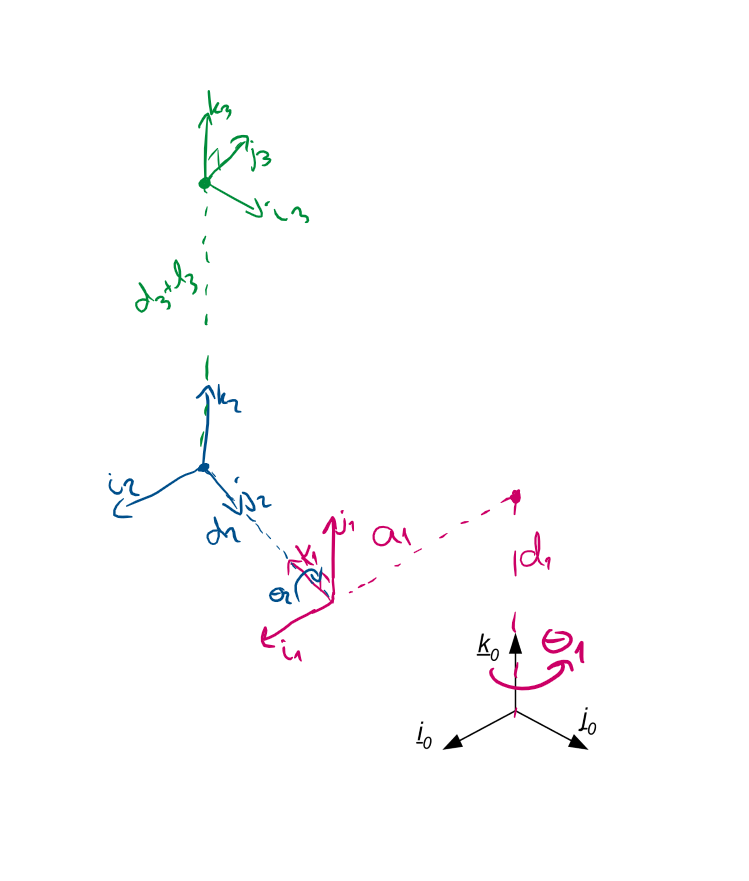
\includegraphics[width = .95\textwidth]{4.PNG}
    \caption{Sketch of ``home'' position based on the DH-table provided}
    \label{fig:4}
\end{figure}
\todo{Find the Jacobian and how to do this}

\section{}
\subsection{}
The different coordinate frames are sketched and the completed table is found in \autoref{fig:5a}. I see now that it should have been in degrees, but I have filled the table with the radian values.   
\begin{figure}[h!]
    \centering
    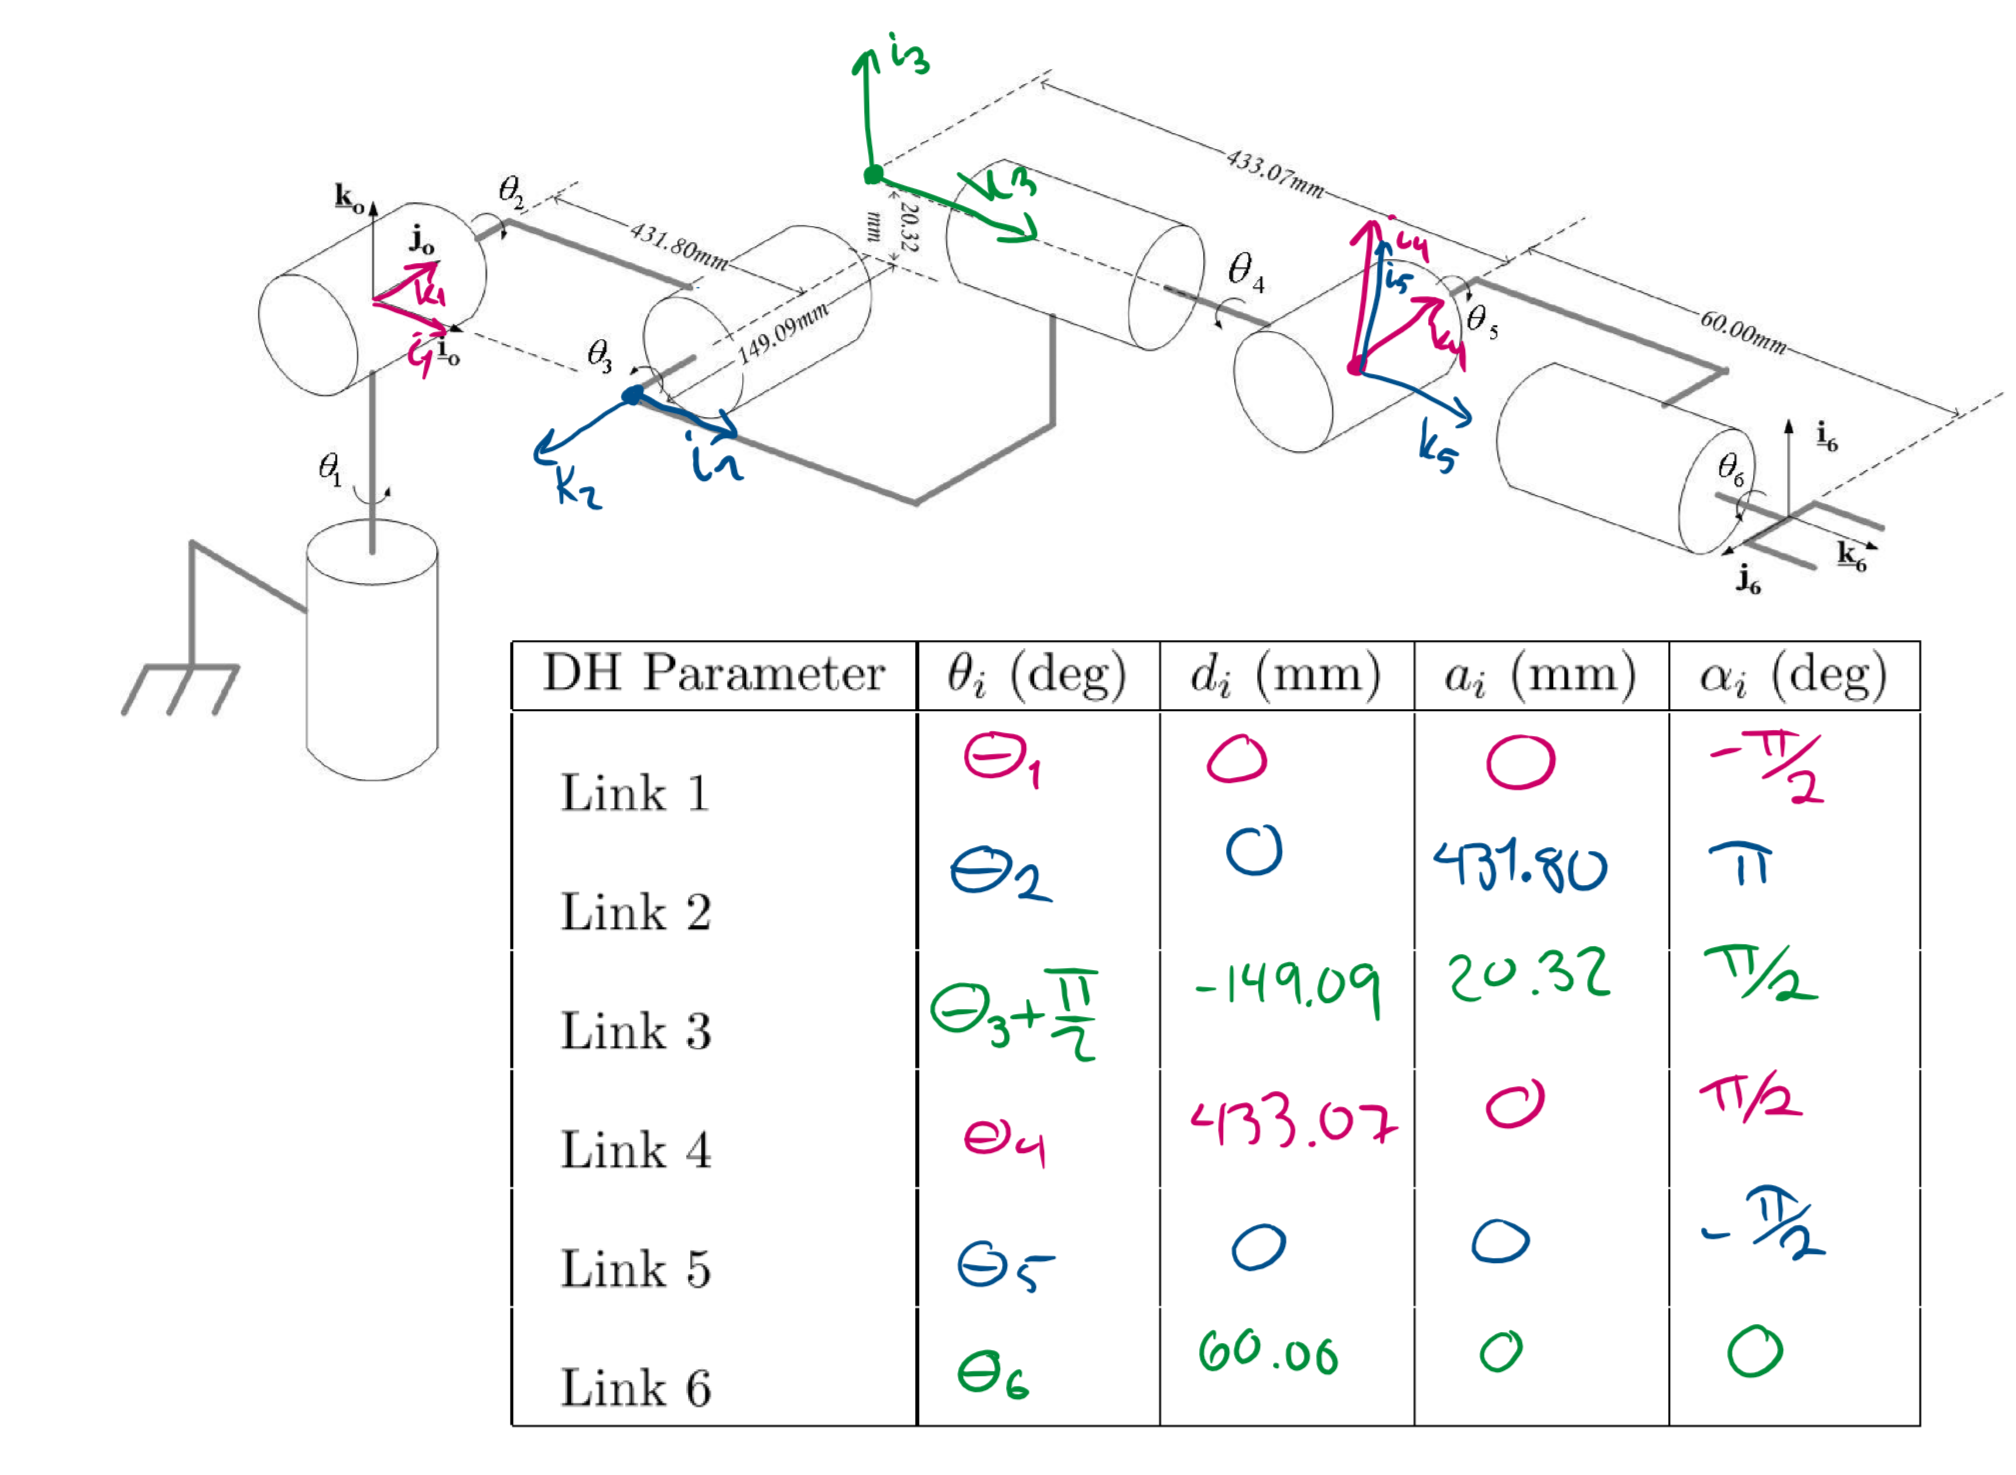
\includegraphics[width = .95\textwidth]{5a.PNG}
    \caption{Sketch of the coordinate frames according to the DH-convention}
    \label{fig:5a}
\end{figure}

\subsection{}
We know that the relationship between base $\{\undertilde{\bm{o}_0} , \underline{C}_0\}$ and the end effector $\{\undertilde{\bm{o}_6} , \underline{C}_6\}$ is given by
\begin{equation}
    \begin{aligned}
        \begin{bmatrix}
            \underline{C}_n & \undertilde{\bm{o}_n} \\
            \bm{0}^\top & 1 
        \end{bmatrix}&=
        \begin{bmatrix}
            \underline{C}_0 & \undertilde{\bm{o}_0} \\
            \bm{0}^\top & 1
        \end{bmatrix} \prescript{0}{}{T}_1(q_1) \prescript{1}{}{T}_2(q_2) \hdots \prescript{n-1}{}{T}_n(q_n) \\
        \implies 
        \begin{bmatrix}
            \underline{C}_6 & \undertilde{\bm{o}_6} \\
            \bm{0}^\top & 1 
        \end{bmatrix}&=
        \begin{bmatrix}
            \underline{C}_0 & \undertilde{\bm{o}_0} \\
            \bm{0}^\top & 1
        \end{bmatrix} \prescript{0}{}{T}_6\\
    \end{aligned}
\end{equation}
where $\prescript{0}{}{T}_6$ is a series of transformations on the form as shown in the first line of \eqref{eq:2a}, and we have the relationship between he base and the end effector. A chain of transformations that give the relationship between  base $\{\undertilde{\bm{o}_0} , \underline{C}_0\}$ and the end effector $\{\undertilde{\bm{o}_6} , \underline{C}_6\}$ on the form presented by Salcudean's example 2.5 is
\begin{equation} \label{eq:5btransformationchain}
    \begin{aligned}
        \underline{C}_1 &= \underline{C}_0\exp\left(\theta_1 \bm{k}\cross\right)\exp\left(-\tfrac{\pi}{2}\bm{i}\cross\right) 
        \quad& \undertilde{\bm{o}_1} &=\undertilde{\bm{o}_0} \\
        \underline{C}_2 &= \underline{C}_1\exp\left(\theta_2 \bm{k}\cross\right)\exp\left(\pi\bm{i}\cross\right) 
        \quad& \undertilde{\bm{o}_2} &=\undertilde{\bm{o}_1} + \underline{C}_1\exp\left(\theta_2 \bm{k}\cross\right)\left(431.80 \bm{i} \right)\si{\mm} \\
        \underline{C}_3 &= \underline{C}_2 \exp\left(\theta_3 \bm{k}\cross\right) \exp\left(\tfrac{\pi}{2}\bm{k}\cross\right)\exp\left(\tfrac{\pi}{2}\bm{i}\cross\right) 
        \quad& \undertilde{\bm{o}_3} &=\undertilde{\bm{o}_2} +  \underline{C}_2\exp\left(\theta_3 \bm{k}\cross\right) \left(-149.09 \bm{k} + 20.32 \bm{j} \right)\si{\mm} \\
        \underline{C}_4 &= \underline{C}_3 \exp\left(\theta_4 \bm{k}\cross\right) \exp\left(\tfrac{\pi}{2}\bm{i}\cross\right) 
        \quad& \undertilde{\bm{o}_4} &=\undertilde{\bm{o}_3} +  \underline{C}_3\exp\left(\theta_4 \bm{k}\cross\right) \left(433.07 \bm{k} \right)\si{\mm} \\
        \underline{C}_5 &= \underline{C}_4 \exp\left(\theta_5 \bm{k}\cross\right) \exp\left(-\tfrac{\pi}{2}\bm{i}\cross\right) 
        \quad& \undertilde{\bm{o}_5} &=\undertilde{\bm{o}_4}\\
        \underline{C}_6 &= \underline{C}_5 \exp\left(\theta_6 \bm{k}\cross\right) 
         \quad& \undertilde{\bm{o}_6} &=\undertilde{\bm{o}_5} + \underline{C}_5\exp\left(\theta_6 \bm{k}\cross\right) \left(60.00 \bm{k} \right)\si{\mm}
    \end{aligned}
\end{equation}

\subsection{}
\todo{Do exercise 5ce}

\subsection{}\label{ssec:5d} %5d
The MATLAB code used to in \autoref{ssec:5d} is listed in \autoref{lst:5d1}. The user is prompted for six joint avariables, and the total homogenous transformation matrix is calculated aswell as the link origins is plotted by using the \mcode{plot3} command. As \autoref{fig:5d1} shows there are 5 different link origins, as expected by \eqref{eq:5btransformationchain} since origin 0 and 1, and 4 and 5 is the same point. There must however be a slight mistake somwhere in my code, as origin 2 gets moved $\sim 2500 \si{\mm}$ insted of $431.8\si{\mm}$, but I can't find it. The other origins does however seem to fit well with what's expected.
\lstinputlisting[style = Matlab-editor, firstline=5, lastline = 50, caption = MATLAB code used to generatehomogenou transformation matrix for angles chosen by the user, captionpos = b, label = lst:5d1]{../../MATLAB/Assignment1/Ex5.m}
\begin{figure}[ht!]
    \centering
    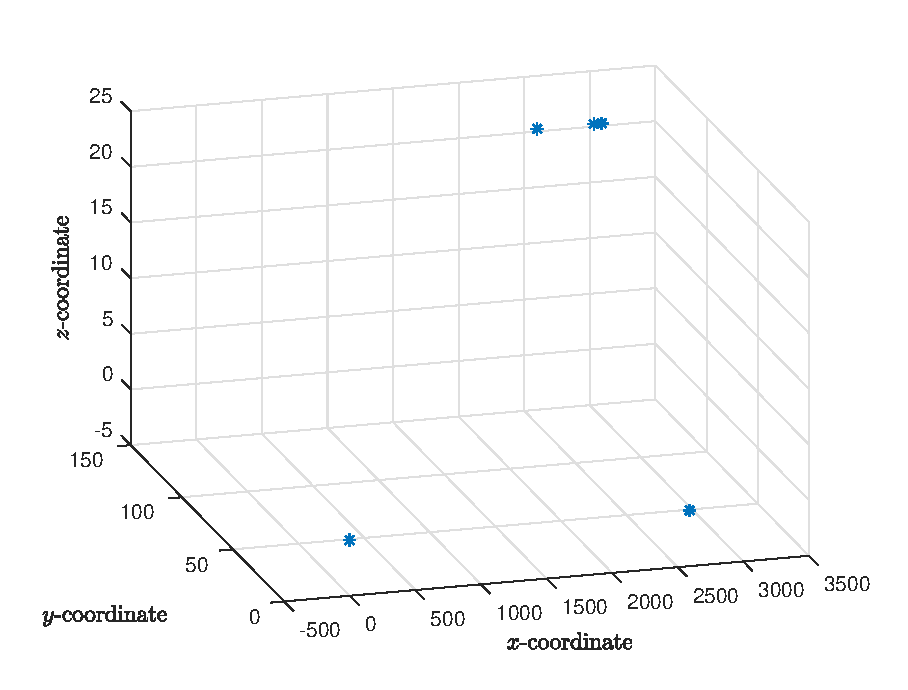
\includegraphics[width = .95\textwidth]{5d1.eps}
    \caption{Location of the link origins with $\theta_i = 0 \enspace \forall i$}
    \label{fig:5d1}
\end{figure}


\end{document}